%%%%\setbeamerfont{itemize/enumerate body}{size*={9}{11}}
%%%%\setbeamerfont{itemize/enumerate subbody}{size*={8}{10}}
%%%%\setbeamerfont{itemize/enumerate subsubbody}{size*={7}{9}}

\frame{%
\frametitle{Handling uncertainty in economic evaluations}
\begin{itemize}
\item Population uncertainty: Sub-group analysis
\item Parameter uncertainty: Sensitivity analysis
\item Structural uncertainty: Sensitivity analysis
\item Collect more data
\item Sensitivity analysis (SA)
\item Deterministic sensitivity analysis
\begin{itemize}
	\item One-way SA
	\item Two-way SA
	\item Scenario analysis (best or worst case, what if..)
\end{itemize}
\item Probabilistic sensitivity analysis (PSA)
\begin{itemize}
	\item Monte Carlo simulation
\end{itemize}
\item Cost-effectiveness acceptability curves (CEAC)
\end{itemize}

}

\frame{%
\frametitle{How robust are health economic evaluations}
\begin{itemize}
\item Do limitations in either the quality or availability of evidence affect the recommended decision?
\item If the decision is not altered despite ‘reasonable’ variations in key assumptions/parameters, then the analysis can be considered to be ‘robust’
\item Two types of uncertainty:
\begin{itemize}
	\item Structural (is the model design correct?)
	\item Parameter (are the values correct?)
\end{itemize}
\item In economic evaluation, some form of sensitivity analysis is frequently carried out in order to allow for uncertainty
\item This uncertainty may be present in the evaluation for several reasons:
\begin{itemize}
	\item Data are unavailable and assumptions are necessary
	\item Available but inaccurate
\end{itemize}
\item In this type of analysis the	values recorded for important parameters are varied, usually one at a time, in order to determine whether the results are sensitive to the assumptions made
\end{itemize}
}

\frame{%
\frametitle{Uncertainty in economic evaluations}
\begin{itemize}
\item Structural: scenario analysis
\item Re-run the analysis with alternate assumptions and model structures
\item Parameter: sensitivity analysis (SA)
\item Re-run the analysis with different parameter values
\item Type of sensitivity analysis:
\begin{itemize}
	\item One-way SA
	\item Multi-way SA
	\item Extreme values SA
	\item Probabilistic SA
\end{itemize}
\end{itemize}
}

\frame{%
\frametitle{Types of sensitivity analysis}
\begin{itemize}
\item Simple sensitivity analysis entails varying one or more of the components of an evaluation to see how it affects the results
\item  Probabilistic sensitivity analysis assigns ranges and distribution to  variables and computer programs  are used to select values at  random from each range and to record the results
\item By using these different methods of sensitivity analysis it is possible to show whether the results of a particular study	over a range of  assumptions or hinge on the accuracy of particular assumptions
\end{itemize}
}


\frame{
\frametitle{A two input example}
\begin{center}\includegraphics[scale=.6]{R/fixed-means}\end{center}
}

\frame{
\frametitle{A two input example}
\begin{center}\includegraphics[scale=.6]{R/fixed-y-min}\end{center}
}

\frame{
\frametitle{A two input example}
\begin{center}\includegraphics[scale=.6]{R/fixed-y-max}\end{center}
}

\frame{
\frametitle{A two input example}
\begin{center}\includegraphics[scale=.6]{R/fixed-x-min}\end{center}
}

\frame{
\frametitle{A two input example}
\begin{center}\includegraphics[scale=.6]{R/fixed-x-max}\end{center}
}

\frame{
\frametitle{A two input example}
\begin{center}\includegraphics[scale=.6]{R/fixed-all}\end{center}
}

\frame{
\frametitle{A two input example}
\begin{center}\includegraphics[scale=.6]{R/full-psa}\end{center}
}


% uncertainty propogation
\frame{
\frametitle{4.\ Uncertainty analysis}
\begin{overprint}
%%%\vspace{7pt}

%%%%%%%%%%%%%%%%%%%%%%%%%%%%%%%%%%%%%%%%%%%%%%%%%
\onslide<1|handout:0>
\fontsize{7}{8}\selectfont
\begin{tabular}{ccc}
\textbf{\blue Parameters} & \textbf{\blue Model structure} & \textbf{\blue Decision analysis} \\
\begin{minipage}[l]{2.5cm}
\begin{center}\includegraphics[scale=.37]{R/means-only}\end{center}
\end{minipage}
&
\begin{minipage}[l]{5cm}
\begin{center}\red{Old chemotherapy}\black\end{center}\vspace{-.5cm}
\begin{center}\includegraphics[scale=.37]{1.introduction-to-health-economic-evaluations/figs/ModelGraph2}\end{center}

\begin{center}\red{New chemotherapy}\black\end{center}\vspace{-.5cm}
\begin{center}\includegraphics[scale=.37]{1.introduction-to-health-economic-evaluations/figs/ModelGraph4}\end{center}
\end{minipage}
&
\begin{minipage}[l]{4cm}
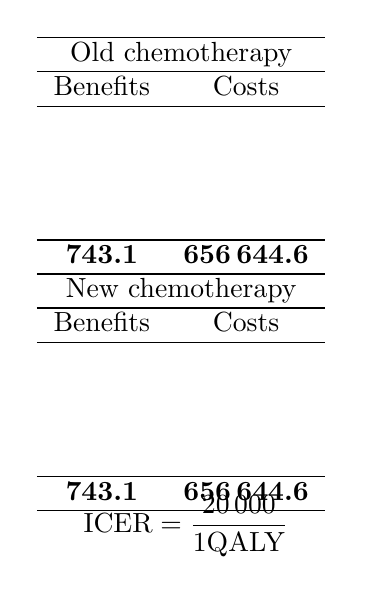
\begin{tikzpicture}
\draw(2.5,2) node[align=center,draw=none]{
\begin{tabular}{cc}
\hline
\multicolumn{2}{c}{Old chemotherapy} \\
\hline
Benefits & Costs \\
\hline 
 &  \\
 &  \\
 &  \\
 &  \\
\hline
\textbf{\white 743.1} & \textbf{\white 656\,644.6} \\
\hline
\end{tabular}
};

\draw(2.5,-1) node[align=center,draw=none]{
\begin{tabular}{cc}
\hline
\multicolumn{2}{c}{New chemotherapy} \\
\hline
Benefits & Costs \\
\hline 
 &  \\
 &  \\
 &  \\
 &  \\
\hline
\textbf{\white 743.1} & \textbf{\white 656\,644.6} \\
\hline
\end{tabular}
};

\draw(2.5,-2.7) node(3){\white $\displaystyle \mbox{ICER} = \frac{\mbox{20\,000}}{\mbox{1QALY}}$\black};
\end{tikzpicture}
\end{minipage}
\end{tabular}


%%%%%%%%%%%%%%%%%%%%%%%%%%%%%%%%%%%%%%%%%%%%%%%%%
\onslide<2|handout:0>
\fontsize{7}{8}\selectfont
\begin{tabular}{ccc}
\textbf{\blue Parameters} & \textbf{\blue Model structure} & \textbf{\blue Decision analysis} \\
\begin{minipage}[l]{2.5cm}
\begin{center}\includegraphics[scale=.37]{R/max-min-pi}\end{center}
\end{minipage}
&
\begin{minipage}[l]{5cm}
\begin{center}\red{Old chemotherapy}\black\end{center}\vspace{-.5cm}
\begin{center}\includegraphics[scale=.37]{1.introduction-to-health-economic-evaluations/figs/ModelGraph2}\end{center}

\begin{center}\red{New chemotherapy}\black\end{center}\vspace{-.5cm}
\begin{center}\includegraphics[scale=.37]{1.introduction-to-health-economic-evaluations/figs/ModelGraph4}\end{center}
\end{minipage}
&
\begin{minipage}[l]{4cm}
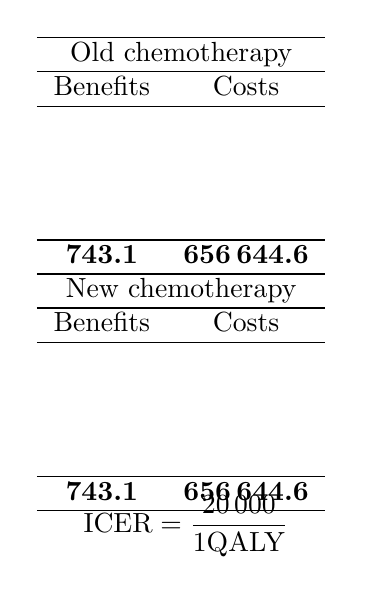
\begin{tikzpicture}
\draw(2.5,2) node[align=center,draw=none]{
\begin{tabular}{cc}
\hline
\multicolumn{2}{c}{Old chemotherapy} \\
\hline
Benefits & Costs \\
\hline 
 &  \\
 &  \\
 &  \\
 &  \\
\hline
\textbf{\white 743.1} & \textbf{\white 656\,644.6} \\
\hline
\end{tabular}
};

\draw(2.5,-1) node[align=center,draw=none]{
\begin{tabular}{cc}
\hline
\multicolumn{2}{c}{New chemotherapy} \\
\hline
Benefits & Costs \\
\hline 
 &  \\
 &  \\
 &  \\
 &  \\
\hline
\textbf{\white 743.1} & \textbf{\white 656\,644.6} \\
\hline
\end{tabular}
};

\draw(2.5,-2.7) node(3){\white $\displaystyle \mbox{ICER} = \frac{\mbox{20\,000}}{\mbox{1QALY}}$\black};
\end{tikzpicture}
\end{minipage}
\end{tabular}

%%%%%%%%%%%%%%%%%%%%%%%%%%%%%%%%%%%%%%%%%%%%%%%%%
\onslide<3|handout:0>
\fontsize{7}{8}\selectfont
\begin{tabular}{ccc}
\textbf{\blue Parameters} & \textbf{\blue Model structure} & \textbf{\blue Decision analysis} \\
\begin{minipage}[l]{2.5cm}
\begin{center}\includegraphics[scale=.37]{R/max-min-rho}\end{center}
\end{minipage}
&
\begin{minipage}[l]{5cm}
\begin{center}\red{Old chemotherapy}\black\end{center}\vspace{-.5cm}
\begin{center}\includegraphics[scale=.37]{1.introduction-to-health-economic-evaluations/figs/ModelGraph2}\end{center}

\begin{center}\red{New chemotherapy}\black\end{center}\vspace{-.5cm}
\begin{center}\includegraphics[scale=.37]{1.introduction-to-health-economic-evaluations/figs/ModelGraph4}\end{center}
\end{minipage}
&
\begin{minipage}[l]{4cm}
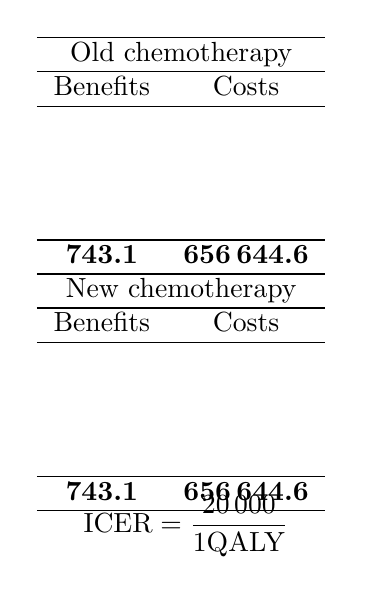
\begin{tikzpicture}
\draw(2.5,2) node[align=center,draw=none]{
\begin{tabular}{cc}
\hline
\multicolumn{2}{c}{Old chemotherapy} \\
\hline
Benefits & Costs \\
\hline 
 &  \\
 &  \\
 &  \\
 &  \\
\hline
\textbf{\white 743.1} & \textbf{\white 656\,644.6} \\
\hline
\end{tabular}
};

\draw(2.5,-1) node[align=center,draw=none]{
\begin{tabular}{cc}
\hline
\multicolumn{2}{c}{New chemotherapy} \\
\hline
Benefits & Costs \\
\hline 
 &  \\
 &  \\
 &  \\
 &  \\
\hline
\textbf{\white 743.1} & \textbf{\white 656\,644.6} \\
\hline
\end{tabular}
};

\draw(2.5,-2.7) node(3){\white $\displaystyle \mbox{ICER} = \frac{\mbox{20\,000}}{\mbox{1QALY}}$\black};
\end{tikzpicture}
\end{minipage}
\end{tabular}

%%%%%%%%%%%%%%%%%%%%%%%%%%%%%%%%%%%%%%%%%%%%%%%%%
\onslide<4|handout:0>
\fontsize{7}{8}\selectfont
\begin{tabular}{ccc}
\textbf{\blue Parameters} & \textbf{\blue Model structure} & \textbf{\blue Decision analysis} \\
\begin{minipage}[l]{2.5cm}
\begin{center}\includegraphics[scale=.37]{R/max-min-gamma}\end{center}
\end{minipage}
&
\begin{minipage}[l]{5cm}
\begin{center}\red{Old chemotherapy}\black\end{center}\vspace{-.5cm}
\begin{center}\includegraphics[scale=.37]{1.introduction-to-health-economic-evaluations/figs/ModelGraph2}\end{center}

\begin{center}\red{New chemotherapy}\black\end{center}\vspace{-.5cm}
\begin{center}\includegraphics[scale=.37]{1.introduction-to-health-economic-evaluations/figs/ModelGraph4}\end{center}
\end{minipage}
&
\begin{minipage}[l]{4cm}
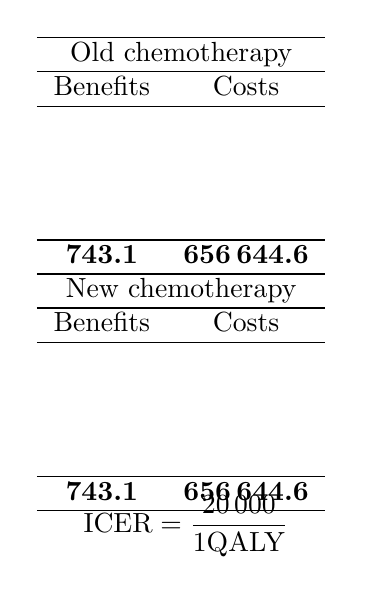
\begin{tikzpicture}
\draw(2.5,2) node[align=center,draw=none]{
\begin{tabular}{cc}
\hline
\multicolumn{2}{c}{Old chemotherapy} \\
\hline
Benefits & Costs \\
\hline 
 &  \\
 &  \\
 &  \\
 &  \\
\hline
\textbf{\white 743.1} & \textbf{\white 656\,644.6} \\
\hline
\end{tabular}
};

\draw(2.5,-1) node[align=center,draw=none]{
\begin{tabular}{cc}
\hline
\multicolumn{2}{c}{New chemotherapy} \\
\hline
Benefits & Costs \\
\hline 
 &  \\
 &  \\
 &  \\
 &  \\
\hline
\textbf{\white 743.1} & \textbf{\white 656\,644.6} \\
\hline
\end{tabular}
};

\draw(2.5,-2.7) node(3){\white $\displaystyle \mbox{ICER} = \frac{\mbox{20\,000}}{\mbox{1QALY}}$\black};
\end{tikzpicture}
\end{minipage}
\end{tabular}

%%%%%%%%%%%%%%%%%%%%%%%%%%%%%%%%%%%%%%%%%%%%%%%%%
\onslide<5|handout:0>
\fontsize{7}{8}\selectfont
\begin{tabular}{ccc}
\textbf{\blue Parameters} & \textbf{\blue Model structure} & \textbf{\blue Decision analysis} \\
\begin{minipage}[l]{2.5cm}
\begin{center}\includegraphics[scale=.37]{R/max-min-cost}\end{center}
\end{minipage}
&
\begin{minipage}[l]{5cm}
\begin{center}\red{Old chemotherapy}\black\end{center}\vspace{-.5cm}
\begin{center}\includegraphics[scale=.37]{1.introduction-to-health-economic-evaluations/figs/ModelGraph2}\end{center}

\begin{center}\red{New chemotherapy}\black\end{center}\vspace{-.5cm}
\begin{center}\includegraphics[scale=.37]{1.introduction-to-health-economic-evaluations/figs/ModelGraph4}\end{center}
\end{minipage}
&
\begin{minipage}[l]{4cm}
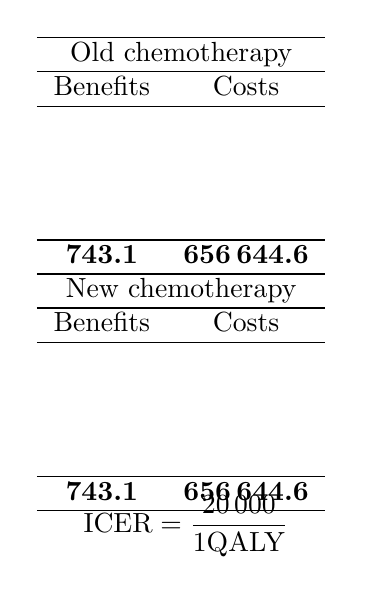
\begin{tikzpicture}
\draw(2.5,2) node[align=center,draw=none]{
\begin{tabular}{cc}
\hline
\multicolumn{2}{c}{Old chemotherapy} \\
\hline
Benefits & Costs \\
\hline 
 &  \\
 &  \\
 &  \\
 &  \\
\hline
\textbf{\white 743.1} & \textbf{\white 656\,644.6} \\
\hline
\end{tabular}
};

\draw(2.5,-1) node[align=center,draw=none]{
\begin{tabular}{cc}
\hline
\multicolumn{2}{c}{New chemotherapy} \\
\hline
Benefits & Costs \\
\hline 
 &  \\
 &  \\
 &  \\
 &  \\
\hline
\textbf{\white 743.1} & \textbf{\white 656\,644.6} \\
\hline
\end{tabular}
};

\draw(2.5,-2.7) node(3){\white $\displaystyle \mbox{ICER} = \frac{\mbox{20\,000}}{\mbox{1QALY}}$\black};
\end{tikzpicture}
\end{minipage}
\end{tabular}

% PSA
%%%%%%%%%%%%%%%%%%%%%%%%%%%%%%%%%%%%%%%
\onslide<6|handout:0>
\fontsize{7}{8}\selectfont
\begin{tabular}{ccc}
\textbf{\blue Parameters} & \textbf{\blue Model structure} & \textbf{\blue Decision analysis} \\
\begin{minipage}[l]{2.5cm}
\begin{center}\includegraphics[scale=.37]{R/psa-1}\end{center}
\end{minipage}
&
\begin{minipage}[l]{5cm}
\begin{center}\red{Old chemotherapy}\black\end{center}\vspace{-.5cm}
\begin{center}\includegraphics[scale=.37]{1.introduction-to-health-economic-evaluations/figs/ModelGraph2}\end{center}

\begin{center}\red{New chemotherapy}\black\end{center}\vspace{-.5cm}
\begin{center}\includegraphics[scale=.37]{1.introduction-to-health-economic-evaluations/figs/ModelGraph4}\end{center}
\end{minipage}
&
\begin{minipage}[l]{4cm}
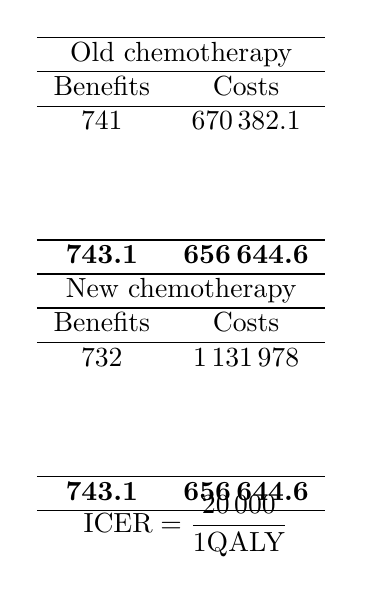
\begin{tikzpicture}
\draw(2.5,2) node[align=center,draw=none]{
\begin{tabular}{cc}
\hline
\multicolumn{2}{c}{Old chemotherapy} \\
\hline
Benefits & Costs \\
\hline 
741 & 670\,382.1 \\
 &  \\
 &  \\
 &  \\
\hline
\textbf{\white 743.1} & \textbf{\white 656\,644.6} \\
\hline
\end{tabular}
};

\draw(2.5,-1) node[align=center,draw=none]{
\begin{tabular}{cc}
\hline
\multicolumn{2}{c}{New chemotherapy} \\
\hline
Benefits & Costs \\
\hline 
732 & 1\,131\,978 \\
 &  \\
 &  \\
 &  \\
\hline
\textbf{\white 743.1} & \textbf{\white 656\,644.6} \\
\hline
\end{tabular}
};

\draw(2.5,-2.7) node(3){\white $\displaystyle \mbox{ICER} = \frac{\mbox{20\,000}}{\mbox{1QALY}}$\black};
%\draw(-5.5,.3) node(4){$\Rightarrow$};
%\draw(-0,.3) node(5){$\Rightarrow$};
\end{tikzpicture}
\end{minipage}
\end{tabular}


%%%%%%%%%%%%%%%%%%%%%%%%%%%%%%%%%%%%%%%
\onslide<7|handout:0>
\fontsize{7}{8}\selectfont
\begin{tabular}{ccc}
\textbf{\blue Parameters} & \textbf{\blue Model structure} & \textbf{\blue Decision analysis} \\
\begin{minipage}[l]{2.5cm}
\begin{center}\includegraphics[scale=.37]{R/psa-2}\end{center}
\end{minipage}
&
\begin{minipage}[l]{5cm}
\begin{center}\red{Old chemotherapy}\black\end{center}\vspace{-.5cm}
\begin{center}\includegraphics[scale=.37]{1.introduction-to-health-economic-evaluations/figs/ModelGraph2}\end{center}

\begin{center}\red{New chemotherapy}\black\end{center}\vspace{-.5cm}
\begin{center}\includegraphics[scale=.37]{1.introduction-to-health-economic-evaluations/figs/ModelGraph4}\end{center}
\end{minipage}
&
\begin{minipage}[l]{4cm}
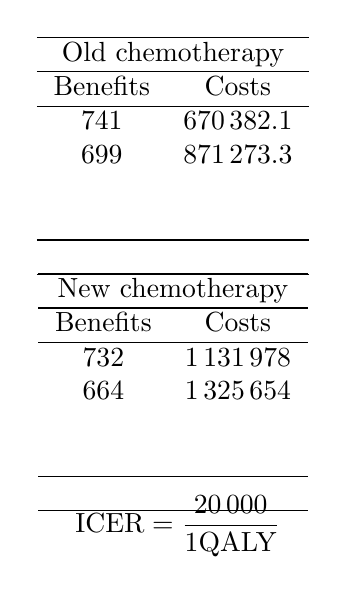
\begin{tikzpicture}
\draw(2.5,2) node[align=center,draw=none]{
\begin{tabular}{cc}
\hline
\multicolumn{2}{c}{Old chemotherapy} \\
\hline
Benefits & Costs \\
\hline 
741 & 670\,382.1 \\
699 & 871\,273.3 \\
 &  \\
 &  \\
\hline
 &  \\
\hline
\end{tabular}
};

\draw(2.5,-1) node[align=center,draw=none]{
\begin{tabular}{cc}
\hline
\multicolumn{2}{c}{New chemotherapy} \\
\hline
Benefits & Costs \\
\hline 
732 & 1\,131\,978 \\
664 & 1\,325\,654 \\
 &  \\
 &  \\
\hline
 &  \\
\hline
\end{tabular}
};

\draw(2.5,-2.7) node(3){\white $\displaystyle \mbox{ICER} = \frac{\mbox{20\,000}}{\mbox{1QALY}}$\black};
%\rput(-5.5,.3){$\Rightarrow$}
%\rput(-0,.3){$\Rightarrow$}
\end{tikzpicture}
\end{minipage}
\end{tabular}

%%%%%%%%%%%%%%%%%%%%%%%%%%%%%%%%%%%%%%%%%%%%%%%%%%%
\onslide<8|handout:1>
\fontsize{7}{8}\selectfont
\begin{tabular}{ccc}
\textbf{\blue Parameters} & \textbf{\blue Model structure} & \textbf{\blue Decision analysis} \\
\begin{minipage}[l]{2.5cm}
\begin{center}\includegraphics[scale=.37]{R/psa-3}\end{center}
\end{minipage}
&
\begin{minipage}[l]{5cm}
\begin{center}\red{Old chemotherapy}\black\end{center}\vspace{-.5cm}
\begin{center}\includegraphics[scale=.37]{1.introduction-to-health-economic-evaluations/figs/ModelGraph2}\end{center}

\begin{center}\red{New chemotherapy}\black\end{center}\vspace{-.5cm}
\begin{center}\includegraphics[scale=.37]{1.introduction-to-health-economic-evaluations/figs/ModelGraph4}\end{center}
\end{minipage}
&
\begin{minipage}[l]{4cm}
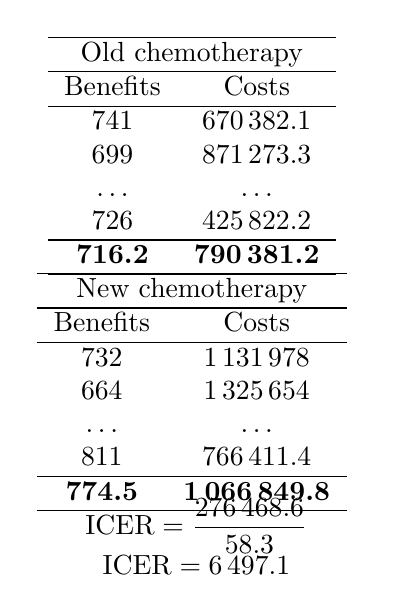
\begin{tikzpicture}
\draw(2.5,2) node[align=center,draw=none]{
\begin{tabular}{cc}
\hline
\multicolumn{2}{c}{Old chemotherapy} \\
\hline
Benefits & Costs \\
\hline 
741 & 670\,382.1 \\
699 & 871\,273.3 \\
$\ldots$ & $\ldots$ \\
726 & 425\,822.2 \\
\hline
\textbf{716.2} & \textbf{790\,381.2} \\
\hline
\end{tabular}
};

\draw(2.5,-1) node[align=center,draw=none]{
\begin{tabular}{cc}
\hline
\multicolumn{2}{c}{New chemotherapy} \\
\hline
Benefits & Costs \\
\hline 
732 & 1\,131\,978 \\
664 & 1\,325\,654 \\
$\ldots$ & $\ldots$ \\
811 & 766\,411.4 \\
\hline
\textbf{774.5} & \textbf{1\,066\,849.8} \\
\hline
\end{tabular}
};

\draw(2.5,-2.7) node(3){$\displaystyle \mbox{ICER} = \frac{\mbox{276\,468.6}}{\mbox{58.3}}$};
\draw(2.5,-3.2) node(3){$\displaystyle \mbox{\white ICER\black} = \mbox{6\,497.1}$};
%%%%
%%%%\rput(2,-2.7){$\displaystyle \mbox{ICER =} \frac{\mbox{276\,468.6}}{\mbox{58.3}}$}
%%%%\rput(2,-3.2){$\displaystyle \mbox{\white ICER\black =} \mbox{ 6\,497.1}$}
%%%%\rput(-5.5,.3){$\Rightarrow$}
%%%%\rput(-0,.3){$\Rightarrow$}
\end{tikzpicture}
\end{minipage}
\end{tabular}

\end{overprint}
}

\frame{
\frametitle{Is this \textit{all} we need? \hspace{0pt plus 1 filll}\small \textit{(see VoI)}}
\only<1-3|handout:1>{
\begin{itemize}
\item The CEAC only deals with the \textbf{\blue probability} of making the ``right decision''
\item But it does not account for the \textbf{\red payoff/penalty} associated with making the ``wrong''~one!
\vspace{10pt}
\item<2-3|handout:1> \textbf{Example 1}: Intervention $t=1$ is the most cost-effective, given current evidence
\begin{itemize}
\item<2-3|handout:1> \myblue $\Pr(\mbox{$t=1$ is cost-effective)}=$ 0.51 \black 
\item<2-3|handout:1> If we get it wrong: Increase in costs = \pounds 3
\item[]<2-3|handout:1> \white If we get it wrong: \black Decrease in effectiveness = 0.000001 QALYs
\item \red Large uncertainty\black/\color{blue!20!black!30!green} negligible consequences \black $\Rightarrow$ \textbf{\color{blue!20!black!30!green}can afford uncertainty}
\end{itemize}
\vspace{5pt}
\item<3|handout:1> \textbf{Example 2}: Intervention $t=1$ is the most cost-effective, given current evidence
\begin{itemize}
\item<3|handout:1> \myblue $\Pr(\mbox{$t=1$ is cost-effective)}=$ 0.999 \black 
\item<3|handout:1> If we get it wrong: Increase in costs = \pounds 1\,000\,000\,000
\item[]<3|handout:1> \white If we get it wrong: \black Decrease in effectiveness = 999999 QALYs
\item<3|handout:1> \color{blue!20!black!30!green} Tiny uncertainty\black/\red dire consequences \black $\Rightarrow$ \amber \textbf{probably should think about~it...}
\end{itemize}
\end{itemize}
}
}

